\begin{frame}[plain]\titlepage
\begin{center}\large Molecular design $\rightarrow$ polymerizable redox centers\end{center}
\end{frame}
\begin{frame}{The target is a redox-active polymer for a flow battery}
\begin{columns}[T]\begin{column}{.48\textwidth}
\begin{block}{Research objective}Choose pendant redox centers that remain useful after monomer functionalization and polymerization.\end{block}
\vspace{.8em}\large Which molecular advantages survive the route to the polymer?
\end{column}\begin{column}{.48\textwidth}
\begin{tikzpicture}[every node/.style={draw=teal,fill=soft,rounded corners,align=center,text width=2.5cm,minimum height=1.2cm,font=\small}]
\node (a) {Redox potential\\Operating window};
\node[right=.3cm of a] (b) {Active loading\\Capacity};
\node[below=.4cm of a] (c) {Charge transfer\\Kinetics};
\node[below=.4cm of b] (d) {Chemical route\\Redox retention};
\end{tikzpicture}
\end{column}\end{columns}
\vfill\footnotesize Molecular screening supplies design hypotheses; polymer accessibility and cycling must be tested.
\end{frame}
\begin{frame}{Start with the monomer synthesis route}
\centering
\begin{tikzpicture}[node distance=.75cm,>=Latex]
\node[draw=teal,fill=soft,rounded corners,text width=3.1cm,minimum height=1.5cm,align=center] (a) {Redox center\\+ \mbox{vinylbenzyl}\\handle};
\node[right=of a,draw=teal,fill=soft,rounded corners,text width=3.1cm,minimum height=1.5cm,align=center] (b) {Functionalized\\vinyl monomer};
\node[right=of b,draw=teal,fill=soft,rounded corners,text width=3.1cm,minimum height=1.5cm,align=center] (c) {Polymer bearing\\redox centers};
\draw[->,thick,teal] (a)--(b);\draw[->,thick,teal] (b)--(c);\end{tikzpicture}
\vspace{1.2em}\begin{block}{The design question}
Which center combines useful redox behavior with a workable route to the polymer?
\end{block}
\vspace{.5em}Potential and capacity guide screening; kinetics and synthesis guide the next tests.
\end{frame}
\begin{frame}{Workflow: from candidate families to synthesis controls}
\centering
\begin{tikzpicture}[node distance=.45cm,>=Latex,every node/.style={font=\small}]
\node[draw=teal,fill=soft,rounded corners,text width=2.65cm,minimum height=1.6cm,align=center] (a) {Build exact\\molecular models};
\node[right=of a,draw=teal,fill=soft,rounded corners,text width=2.65cm,minimum height=1.6cm,align=center] (b) {Sample\\conformers};
\node[right=of b,draw=teal,fill=soft,rounded corners,text width=2.65cm,minimum height=1.6cm,align=center] (c) {Compute solution\\redox states};
\node[right=of c,draw=teal,fill=soft,rounded corners,text width=2.65cm,minimum height=1.6cm,align=center] (d) {Compare models\\and select\\controls};
\draw[->,thick,teal] (a)--(b);\draw[->,thick,teal] (b)--(c);\draw[->,thick,teal] (c)--(d);
\end{tikzpicture}
\vspace{1em}\begin{columns}[T]\begin{column}{.47\textwidth}
\textbf{Chemical space}\\Diimides; benzoquinones (BQ) and anthraquinones (AQ); viologens; positive-side controls.
\end{column}\begin{column}{.47\textwidth}
\textbf{Selection}\\Potential, nominal capacity, kinetic evidence and synthetic route.
\end{column}\end{columns}
\vfill\footnotesize Finished fields enter comparisons after their checks. Missing properties remain pending.
\end{frame}
\begin{frame}{Method: compare free energies of matched solution states}
\centering\begin{tikzpicture}[node distance=1.2cm,>=Latex]
\node[draw=teal,fill=soft,rounded corners,align=center,minimum width=2.3cm,minimum height=1.1cm] (a) {$M^{q}$\\$G_0$};
\node[right=of a,draw=teal,fill=soft,rounded corners,align=center,minimum width=2.3cm,minimum height=1.1cm] (b) {$M^{q-1}$\\$G_1$};
\node[right=of b,draw=teal,fill=soft,rounded corners,align=center,minimum width=2.3cm,minimum height=1.1cm] (c) {$M^{q-2}$\\$G_2$};
\draw[->,thick,teal] (a)--node[above] {$+e^-$}(b);\draw[->,thick,teal] (b)--node[above] {$+e^-$}(c);
\end{tikzpicture}
\vspace{.7em}\begin{columns}[T]\begin{column}{.55\textwidth}
\small\begin{tabular}{@{}ll@{}}\textbf{Geometry} & r2SCAN-D4 / SVP(D) \\ \textbf{Electronic energy} & $\omega$B97M-V / TZVPD \\ \textbf{Environment} & SMD acetonitrile \\ \textbf{Thermal correction} & Native Hessian, 298 K \\ \end{tabular}
\end{column}\begin{column}{.43\textwidth}
\small $G=E_{\rm electronic}+G_{\rm thermal}$\\[.6em]
Redox potentials from $\Delta G$, referenced consistently to Fc/Fc$^+$.\\[.6em]
Nominal capacity: $Q=\dfrac{nF}{3.6M}$.
\end{column}\end{columns}
\vfill\footnotesize Charge states preserve the declared molecular graph. Stationarity, derivatives, spin and reference consistency are checked separately.
\end{frame}
\begin{frame}{Quinone models lead nominal capacity}
\centering
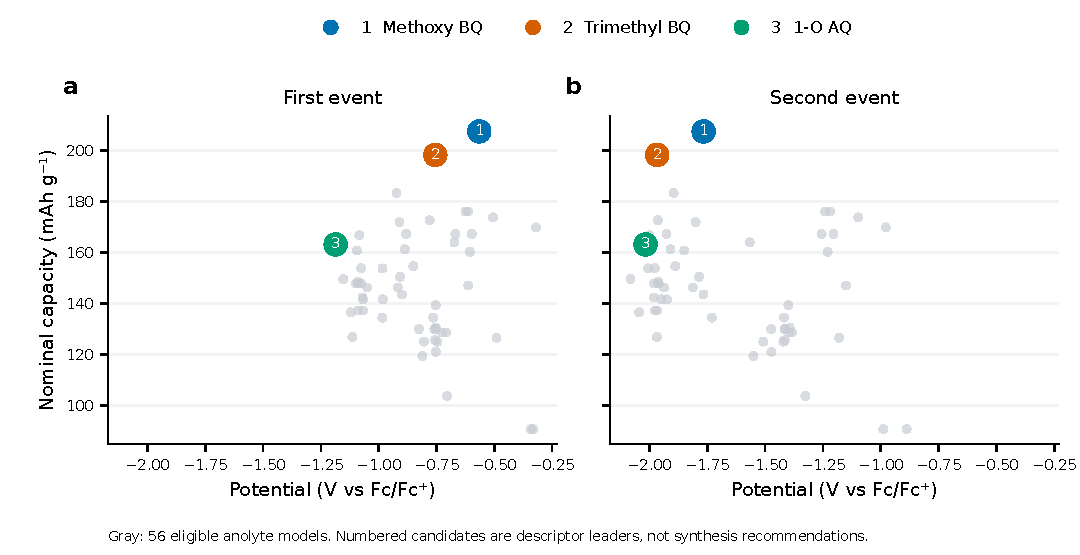
\includegraphics[width=.98\linewidth,height=.70\textheight,keepaspectratio]{../results/candidates/figures/plots/redox_capacity.pdf}
\par\smallskip\raggedright\textcolor{teal}{\textbf{The two BQ models reach 207.5 and 198.3 mAh g$^{-1}$.}}
\par\smallskip\footnotesize 75 designs; 61 checked ladders. Nominal capacity excludes polymer and counterions.
\end{frame}
\begin{frame}{Core topology changes NDI reduction potentials}
\centering
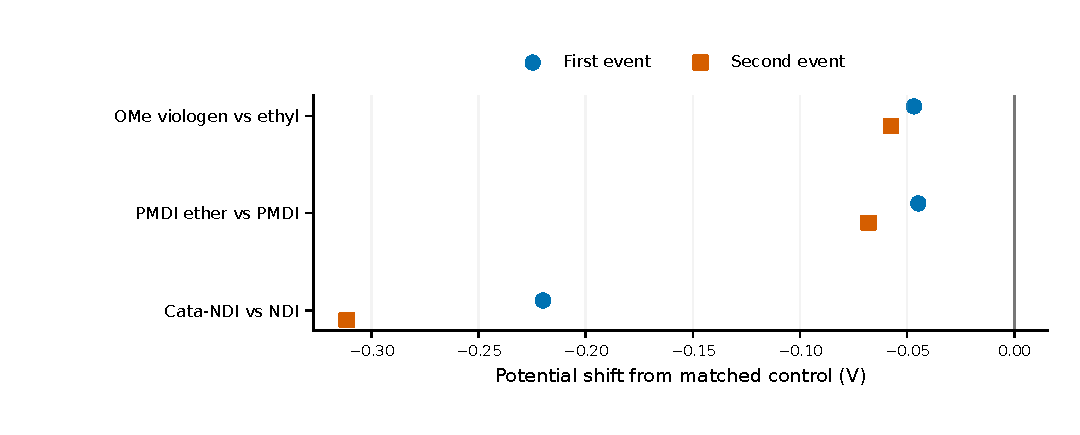
\includegraphics[width=.98\linewidth,height=.70\textheight,keepaspectratio]{../results/candidates/figures/plots/new_candidate_shifts.pdf}
\par\smallskip\raggedright\textcolor{teal}{\textbf{NDI core topology shifts $E_1$ by -0.220 V and $E_2$ by -0.312 V.}}
\par\smallskip\footnotesize Matched model differences in MeCN; voltage shifts alone do not establish battery performance.
\end{frame}
\begin{frame}{SA is a separate filter for candidate choice}
\centering
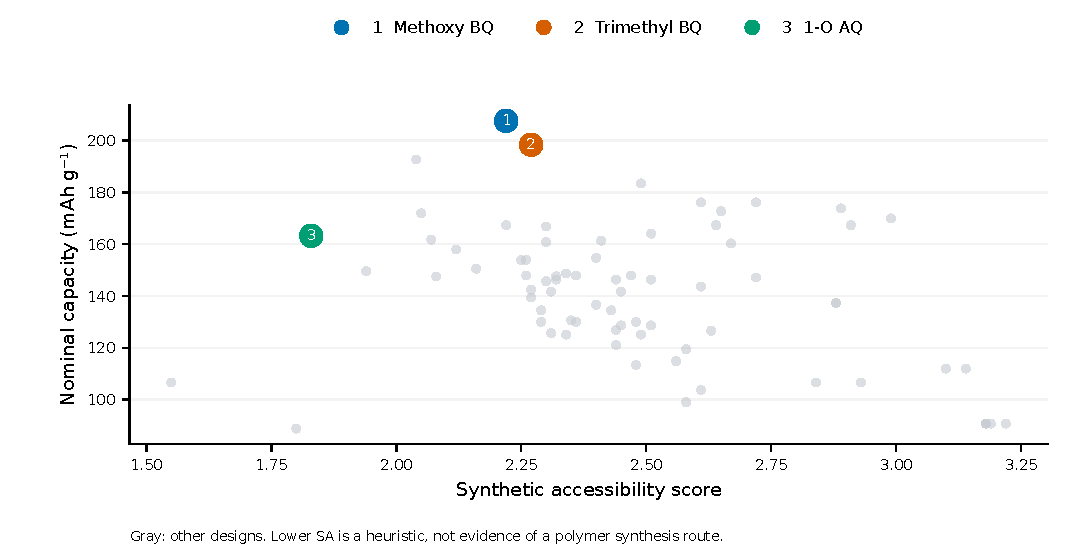
\includegraphics[width=.98\linewidth,height=.70\textheight,keepaspectratio]{../results/candidates/figures/plots/synthesis_tradeoff.pdf}
\par\smallskip\raggedright\textcolor{teal}{\textbf{High capacity and low SA do not establish a polymerization route.}}
\par\smallskip\footnotesize SA is heuristic; polymerization compatibility and redox retention remain untested.
\end{frame}
\begin{frame}{Capacity leaders and the first monomer pilot differ}
\centering
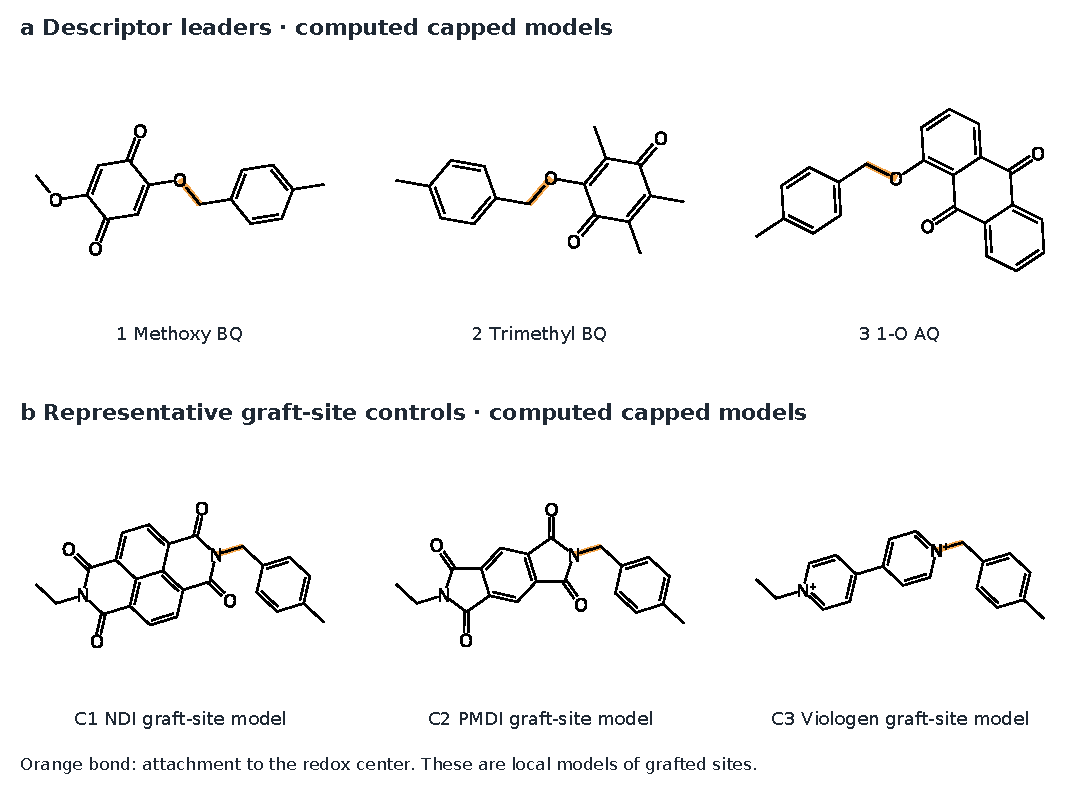
\includegraphics[width=.98\linewidth,height=.70\textheight,keepaspectratio]{../results/candidates/figures/structures/candidate_structures.pdf}
\par\smallskip\raggedright\textcolor{teal}{\textbf{The pilot tests NDI, PMDI and viologen with the actual vinyl handle.}}
\par\smallskip\footnotesize NDI: naphthalene diimide. PMDI: pyromellitic diimide. Vinyl potentials remain pending.
\end{frame}
\begin{frame}{The vinyl group carries a small nominal capacity penalty}
\centering\renewcommand{\arraystretch}{1.65}
\begin{tabular}{@{}lrr@{}}\toprule
Core & Capped model & Vinyl monomer \\
& \multicolumn{2}{c}{Nominal capacity / mAh g$^{-1}$} \\ \midrule
NDI / ethyl & 134.5 & 130.6 \\
PMDI / ethyl & 153.9 & 148.7 \\
Viologen / ethyl & 184.6 & 177.2 \\
\bottomrule\end{tabular}
\vspace{1em}\begin{block}{The larger open question is electronic}
How much does the vinyl-bearing structure shift the redox potentials?
\end{block}
\footnotesize Same declared two-electron count; one added carbon. Stoichiometric capacities exclude counterions and polymer. Vinyl potentials remain pending.
\end{frame}
\begin{frame}{Three findings guide the next experiments}
\begin{block}{Capacity}\textbf{Substituted BQ models lead the current nominal-capacity screen.}\end{block}
\begin{block}{Voltage tuning}\textbf{NDI core topology provides a clear matched computational contrast.}\end{block}
\begin{block}{Synthesis direction}\textbf{Compare exact vinyl NDI, PMDI and viologen before committing to polymer synthesis.}\end{block}
\vfill\footnotesize Next decision: combine monomer redox properties, qualified kinetics and polymerization evidence. Solubility and cycling performance remain unmeasured for these exact targets.
\end{frame}
